\documentclass[12pt]{article}

%%%%%%%%%%%%%%%%%%%%%%
%%%%%%% PACAKAGES %%%%%%%
%%%%%%%%%%%%%%%%%%%%%


%%%%%%%%%%%%% GRAPHICS/FONTS
\usepackage{amsmath,amsfonts,amssymb,graphicx,tikz-cd,pgfplots}

%%%%%%%%%%%%%% FORMATTING
\usepackage{geometry,titlesec,hyperref,xhfill,setspace,float,fancyhdr}

%%%%%%%%DEFINING COMMANDS
\usepackage{xifthen}

\usepackage{parskip}

%%%%%%%%%TIKZ STUFF
\usetikzlibrary{positioning,calc}
\usetikzlibrary{decorations.markings}
\usepgfplotslibrary{polar}
\usepgflibrary{shapes.geometric}
\usepgfplotslibrary{fillbetween}

%%%%%%FOR THE GRAPHS
\pgfplotsset{my style/.append style={axis x line=middle, axis y line=
middle, xlabel={$x$}, ylabel={$y$}, axis equal }}

%%%%%%MARGINS
\geometry{
    letterpaper,
    left=0.25in,
    right=0.25in,
    top=0.25in,
    bottom=0.75in
}

%%%%%%MAKES THE HEADER AND FOOTER FANCY
\fancyhf{}
\renewcommand{\headrulewidth}{0pt}
\pagestyle{fancy}

%%%%%%%%%%%%%%%%%%%%%%
%%%%%%% COMMANDS %%%%%%%
%%%%%%%%%%%%%%%%%%%%%
\newcommand{\underscore}{\underline{\hspace{2mm}}}
\newcommand{\Z}{\mathbb{Z}}
\newcommand{\N}{\mathbb{N}}
\newcommand{\Q}{\mathbb{Q}}
\newcommand{\C}{\mathbb{C}}
\newcommand{\R}{\mathbb{R}}
\newcommand{\Aut}{\text{Aut}}
\newcommand{\GL}{\text{GL}}
\newcommand{\SL}{\text{SL}}
\newcommand{\SO}{\text{SO}}
\newcommand{\PGL}{\text{PGL}}
\newcommand{\Stab}{\text{Stab}}
\newcommand{\End}{\text{End}}
\newcommand{\ad}{\text{ad}}
\newcommand{\lra}{\longrightarrow}

\newcommand{\gl}{\mathfrak{gl}}
\newcommand{\sll}{\mathfrak{sl}}
\newcommand{\pgl}{\mathfrak{pgl}}
\newcommand{\g}{\mathfrak{g}}
\newcommand{\h}{\mathfrak{h}}
\newcommand{\n}{\mathfrak{n}}
\newcommand{\la}{\mathfrak{a}}
\newcommand{\lb}{\mathfrak{b}}
\newcommand{\so}{\mathfrak{so}}


\newcommand{\RP}{\mathbb{R}P}
\newcommand{\K}{\emph{K}}

\renewcommand{\H}{\mathbb{H}}


\newcommand{\ihat}{\hat{\imath}}
\newcommand{\jhat}{\hat{\jmath}}
\newcommand{\khat}{\hat{k}}

\newcommand{\qed}{\quad \blacksquare}

%TEXT COMMAND
\newcommand{\T}[1][]{\text{#1}}
\newcommand{\TB}[1][]{\mathbb{#1}}

\newcommand{\abs}[1]{\left\vert #1 \right\vert}
\newcommand{\brak}[1]{\left\langle #1 \right\rangle}

\newcommand{\xlra}[1][]{%
  \ifthenelse{\isempty{#1}}%
    {\xrightarrow{\phantom{,,,,,,}}}% if #1 is empty
    {\xrightarrow{\phantom{,,}#1\phantom{,,}}}% if #1 is not empty
}


%%%%%%%%%%%%%%%%%%%%%%%%%%%%%%%%%%%%%%%%
%%%%%%%%BEGINNING OF ACTUAL DOCUMENT %%%%%%%%%%
%%%%%%%%%%%%%%%%%%%%%%%%%%%%%%%%%%%%%%%%



%%%%TITLE______REMEMBER TO REGULARLY CHANGE THIS!!!!
\title{Math 1820A Spring 2024 - Homework 8}
\date{}

\begin{document}
\maketitle
\vspace{-0.5in}
%%%%%%%%%%%%%%%%
\begin{spacing}{1.5}
\noindent \textbf{Instructions:}  This assignment is worth twenty points.  Please complete the following problems assigned below.  Submissions with insufficient explanation may lose points due to a lack of reasoning or clarity.  If you are handwriting your work, please ensure it is readable and well-formatted for the grader.

Be sure when uploading your work to \textbf{assign problems to pages}.  Problems with pages not assigned to them \textbf{may not be graded}.  
\end{spacing}




%%%%%%%%%%%%%%%%%%
\vspace{10mm}\noindent
\textbf{Textbook Problems: }  

\noindent
\textbf{Additional Problems:}   For these problems let $\H$ denote the algebra of Hamiltonians and $\H^{\times}$ denote all the non-zero elements as a \emph{group} under multiplication.  For the context of this homework, assume a `rotation' is orientation preserving, and a `reflection' is preserves a codimension 1 subspace.  By a circle on an $n$-sphere we mean the intersection of an affine plane with $S^{n}$.  By a circle in $\R^{n}$ we mean a typical Euclidean circle, or, also a line. 

\pagebreak 
1.  Let $\phi: S^{3} \times S^{3} \lra \SO(4,\R)$ be the homomorphism taking a pair of unit quaternions $(p,q)$ to $L_{p}\circ R_{q^{-1}} : \H \lra \H$ as in class.  Determine the kernel of this map.  (Note this determines the fundamental group of $\SO(4,\R)$ up to isomorphism). 

    \color{blue}
        First suppose that 
        \[p = a + b\ihat + c\jhat + d\khat = 1\]
        Then 
        \[\phi(p, q) = \phi(1, q) = R_{q^{-1}} = \begin{pmatrix}
            w & x & y & z \\
            -x & w & -z & y \\
            -y & z & w & -x \\
            -z & -y & x & w
        \end{pmatrix}\] 
        this is $I_4$ iff $q = 1$. Similarly, if $p = -1$, then 
        \[\phi(-1, q) = -R_{q^{-1}} = -R_{\bar q} \implies q = -1\]

        Now suppose instead that $q = 1$. Then 
        \[\phi(p, 1) = L_p = \begin{pmatrix}
            a & -b & -c & -d \\
            b & a & -d & c \\
            c & d & a & -b \\
            d & -c & b & a
        \end{pmatrix}\]
        Again, this is $I_4$ iff $p = 1$. Further, 
        \[\phi(p, -1) = L_p \circ -I_4 = -L_p \implies p = -1\] 

        Therefore, we have $\{(1, 1), (-1, -1)\} \subset \ker \phi$.

        Now consider the general case. Let $p = a + b\ihat + c\jhat + d\khat$ and $q = w + x \ihat + y \jhat + z \khat$ be two unit quaternions. Then we have 
        \begin{align*}
            L_p &\sim \begin{pmatrix}
                a & -b & -c & -d \\
                b & a & -d & c \\
                c & d & a & -b \\
                d & -c & b & a
            \end{pmatrix}\\ 
            R_{q^{-1}} = R_{\bar q} &\sim \begin{pmatrix}
                w & x & y & z \\
                -x & w & -z & y \\
                -y & z & w & -x \\
                -z & -y & x & w
            \end{pmatrix}
        \end{align*}
        so 
        \begin{align*}
            \phi(p,q) &= L_p \circ R_{q^{-1}}\\
            &= \begin{pmatrix}
                a & -b & -c & -d \\
                b & a & -d & c \\
                c & d & a & -b \\
                d & -c & b & a
            \end{pmatrix} \begin{pmatrix}
                w & x & y & z \\
                -x & w & -z & y \\
                -y & z & w & -x \\
                -z & -y & x & w
            \end{pmatrix}\\ 
            &= \begin{pmatrix}
                a\,w+b\,x+c\,y+d\,z & a\,x-b\,w-c\,z+d\,y & a\,y-c\,w+b\,z-d\,x & a\,z-b\,y+c\,x-d\,w\\
                b\,w-a\,x-c\,z+d\,y & a\,w+b\,x-c\,y-d\,z & b\,y-a\,z+c\,x-d\,w & a\,y+c\,w+b\,z+d\,x\\
                c\,w-a\,y+b\,z-d\,x & a\,z+b\,y+c\,x+d\,w & a\,w-b\,x+c\,y-d\,z & c\,z-b\,w-a\,x+d\,y\\
                c\,x-b\,y-a\,z+d\,w & b\,z-c\,w-a\,y+d\,x & a\,x+b\,w+c\,z+d\,y & a\,w-b\,x-c\,y+d\,z
            \end{pmatrix}
        \end{align*}
        
        To find the kernel of $\phi$, we need to find all $(p,q)$ such that $\phi(p,q) = I_4$. 

        Let's consider just the diagonal entries first: 
        \[\begin{cases}
            aw + bx + cy + dz = 1\\
            aw + bx - cy - dz = 1\\
            aw - bx + cy - dz = 1\\
            aw - bx - cy + dz = 1
        \end{cases}\]

        Which allows us to write 
        \[\begin{pmatrix}
            1 & 1 & 1 & 1\\
            1 & 1 & -1 & -1\\
            1 & -1 & 1 & -1\\
            1 & -1 & -1 & 1
        \end{pmatrix} \begin{pmatrix}
            aw\\bx\\ cy\\ dz
        \end{pmatrix} = \begin{pmatrix}
            1\\1\\1\\1
        \end{pmatrix} \implies \begin{pmatrix}
            aw\\bx\\cy\\dz
        \end{pmatrix} = \begin{pmatrix}
            1\\0\\0\\0
        \end{pmatrix}\]

        Therefore, we have the conditions 
        \begin{gather*}
            a^2 + b^2 + c^2 + d^2 = 1\\ 
            w^2 + x^2 + y^2 + z^2 = 1\\ 
            aw = 1\\ 
            bx = cy = dz = 0
        \end{gather*}

        Suppose WLOG that $x, y, z \neq 0$. Then $b = c = d = 0$ so the norm of $p$ is $a^2 = 1$ so $a = \pm 1$. But these are just our early cases $\phi(1, q)$ and $\phi(-1, q)$.
        
        The last case to consider is when only one of $x, y, z$ is zero forcing the complementary two of $b, c, d$ to be $0$ (or vice versa).
        
        WLOG, suppose $x = 0$ and $y, z \neq 0$. Then $c = d = 0$ so $a^2 + b^2 = 1$ but this implies $a < 1$ (if $b \neq 0$) and similar argument shows $w < 1$ so $aw < 1$ which is a contradiction.

        Therefore, 
        \[\boxed{\ker \phi = \{(1, 1), (-1, -1)\}}\]
    \color{black}


\pagebreak 
2.  Recall from Homework 8, we embedded $S^{3} \subset \GL(4,\R)$ via the left-multiplication representation.  Denote the image of this homomorphism by $\mathcal{H}$ and its Lie-algebra by $\h$.  The Euler-Rodrigues theorem yields a surjective Lie-group homomorphism from $\mathcal{H}$ to $\SO(3,\R)$ with finite kernel.  On the level of Lie-algebras this an isomorphism given by $\psi: \h \lra \mathfrak{so}(3,\R)$ via
\[
\phi\left(
\begin{array}{cccc}
 0 & -a & -b & -c \\
 a & 0 & -c & b \\
 b & c & 0 & -a \\
 c & -b & a & 0 \\
\end{array}
\right) = \left(
\begin{array}{ccc}
 0 & -2 c & 2 b \\
 2 c & 0 & -2 a \\
 -2 b & 2 a & 0 \\
\end{array}
\right)
\]
Using $\psi$, and our homomorphism from Problem 1, construct an isomorphism between $\mathfrak{so}(3,\R) \oplus \mathfrak{so}(3,\R)$ and $\mathfrak{so}(4,\R)$.  

    \color{blue}
        From the problem statement and the isomorphism found in HW 8, we have the following commutative diagram:
        \[\begin{tikzcd}
            S^3 \arrow{r}{L_q} & \mathcal{H} \subset \GL(4, \R) \arrow{d} \arrow[two heads]{r}{\Psi} & \SO(3, \R) \arrow{d}\\ 
            & \h \arrow{d} \arrow[two heads]{r}{\psi} & \so(3, \R)\\
            & \h/Z(\h) \arrow{ur}{\simeq}
        \end{tikzcd}\]

        In class, we proved that $\phi: S^3 \times S^3 \to \SO(4, \R)$ given by $(p, q) \mapsto (L_p \circ R_{q^{-1}})$ is a surjective homomorphism.
        
        In problem 1, we found that $\ker \phi = \{(1, 1), (-1, -1)\} = \Z_2 \times \Z$. Obviously, this is a normal subgroup so we may quotient by it. 

        Therefore, by the first isomorphism theorem, we have that 
        \[(S^3 \times S^3)/(\Z_2 \times \Z_2) \simeq \SO(4, \R)\]

        From the spin double cover of $\SO(3, \R)$ we also have that $S^3/\Z_2 \simeq \SO(3, \R)$. 

        Therefore, 
        \begin{align*}
            (S^3 \times S^3)/(\Z_2 \times \Z_2) &\simeq S^3/\Z_2 \times S^3/\Z_2 \\ 
            &\implies \SO(3, \R) \times \SO(3, \R) \simeq \SO(4, \R)
        \end{align*}        

        Since we have an isomorphism on the Lie group level, we have the isomorphism on the lie algebra level and 
        \[\so(3, \R) \oplus \so(3, \R) \simeq \so(4, \R)\]
        as desired. $\qed$
    \color{black}

\pagebreak 


3.  Recall the construction of stereographic projection in class.  Let $S^{2} \subset \R^{3}$ be the sphere defined by the set of all $(x,y,z) \in \R^{3}$ for which $x^{2} + y^{2} + (z-1)^{2} = 1$.  Denote the north pole by $N = (0,0,2)$.  For each point $p \in S^{2}\setminus N$, construct the line from $N$ to $p$.  This line must intersect the plane $z = 0$ at a unique point.  Write out an explicit expression for this. 

        \color{blue}
            Let $p = (p_1, p_2, p_3)$. Then, in vector form, the line from $N$ to $p$ is given by
            \[\vec v = \vec N + t(\vec p - \vec N) = (0, 0, 2) + t(p_1, p_2, p_3 - 2)\]

            As this line must intersect the plane $z = 0$, we have a system of equations 
            \[\begin{cases}
                x = p_1 t\\ 
                y = p_2 t\\ 
                0 = 2 + (p_3 - 2)t 
            \end{cases}\] 

            Thus, to find the image of $p$ under stereographic projection given a point $(p_1, p_2, p_3)$, we have 
            \[\boxed{(x, y) = \left(-\frac{2p_1}{p_3 - 2}, -\frac{2p_2}{p_3 - 2}\right)}\]
        \color{black}


\pagebreak
4.  Prove that stereographic projection $S^{2}\setminus N \lra \R^{2}$ takes circles on the sphere to circles in $\R^{2}$ (here a circle in $\R^{2}$ can be a line).  Draw some pictures of circles on the sphere getting projected to lines in $\R^{2}$, and be sure to include a circle through $N$ on $S^{2}$. 

    \color{blue}
        Let $c$ be a circle on $S^2$. Denote the plane in $\R^3$ containing $c$ by $P$. Therefore, 
        \[c = \{(i, j, k) \in \R^3 \; | \; (i, j, k) \in S^2 \cap P\}\]

        We can write $P$ in terms of constants 
        \[Ai + Bj + Ck + D = 0\]

        Since the stereographic projection $S^2/N \to \R^2$ is a bijection, we can consider its inverse image: 
        \[f^{-1}(x, y) = \left(\frac{2x}{x^2 + y^2 + 1}, \frac{2y}{x^2 + y^2 + 1}, \frac{x^2 + y^2 - 1}{x^2 + y^2 + 1}\right)\] 

        If a point $(x, y) \in \R^2$ is a projection of a point on $c$, its preimage must lie in $S^2 \cap P$: 
        \[\begin{cases}
            A\left(\frac{2x}{x^2 + y^2 + 1}\right) + B\left(\frac{2y}{x^2 + y^2 + 1}\right) + C\left(\frac{x^2 + y^2 - 1}{x^2 + y^2 + 1}\right) + D =0\\ 
            \left(\frac{2x}{x^2 + y^2 + 1}\right)^2 + \left(\frac{2y}{x^2 + y^2 + 1}\right)^2 + \left(\frac{x^2 + y^2 - 1}{x^2 + y^2 + 1}\right)^2 = 1
        \end{cases}\]

        Rearranging the first equation,
        \begin{gather*}
            A\left(\frac{2x}{x^2 + y^2 + 1}\right) + B\left(\frac{2y}{x^2 + y^2 + 1}\right) + C\left(\frac{x^2 + y^2 - 1}{x^2 + y^2 + 1}\right) + D =0\\ 
            2xA + 2yB + (x^2 + y^2 - 1)C + D(x^2 + y^2 + 1) = 0\\
            2xA + 2yB + (x^2 + y^2)(C + D) = C - D
        \end{gather*}

        For all circles with $N \notin c$ so $C + D \neq 0$, we can take 
        \begin{gather*}
            \frac{2xA}{C + D} + \frac{2yB}{C + D} + x^2 + y^2 = \frac{C - D}{C + D}\\ 
            \left(x + \frac{A}{C + D}\right)^2 + \left(y + \frac{B}{C  +D}\right)^2 = \frac{A^2 + B^2 + C^2 - D^2}{(C^2 - D^2)}
        \end{gather*}
        which is the equation for a circle centered at $\left(-\frac{A}{C + D}, -\frac{B}{C + D}\right)$ with radius $\sqrt{\frac{A^2 + B^2 + C^2 - D^2}{(C^2 - D^2)}}$.

        If $N = (0, 0, 1) \in c$, then $A(0) + B(0) + C(1) + D = 0 \implies C + D = 0$ which defines a line. Therefore, the circle containing $N$ is projected to a line (a general circle). 

        Therefore, the stereographic projection takes circles on the sphere to circles in $\R^2$.
        
        \vspace*{10pt}
        \hrule 
        \vspace*{10pt}

        Using Python and Problem 3, I generated the following diagrams. In each, the left shows the sphere $x^{2} + y^{2} + (z-1)^{2} = 1$. with North Pole marked in red. The circle on the sphere is simulated by 50 points (marked in blue). Their projections are shown in red on the left diagram. The right diagram is an image of the XY-plane containing only the images of the projected points. 

        First, here is the equator on the sphere ($\phi = \pi/2$): 
        \begin{center}
        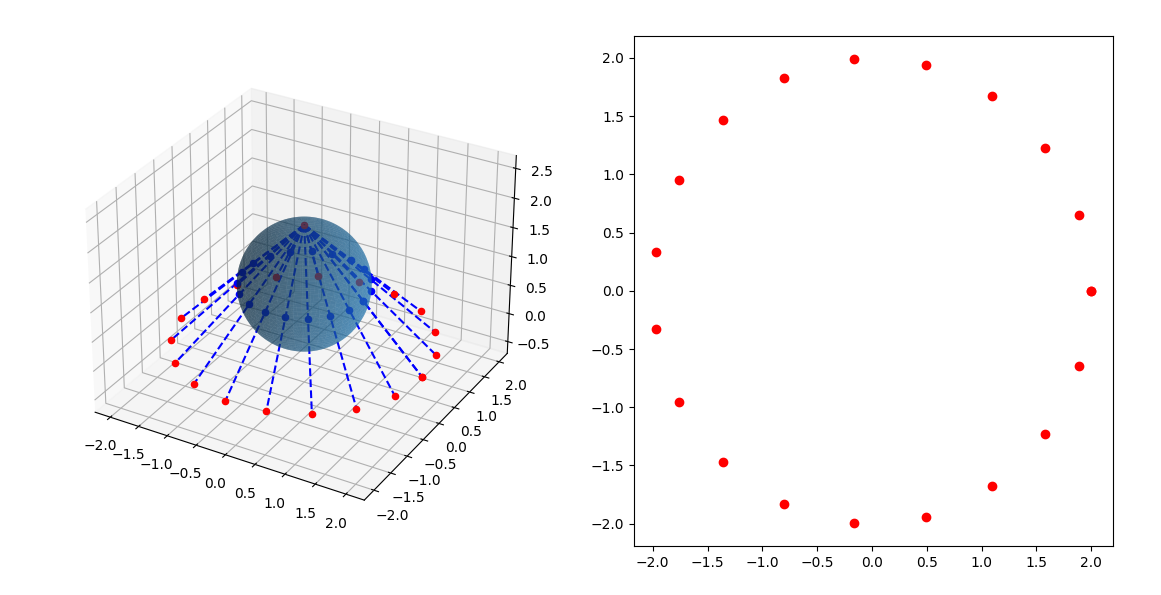
\includegraphics[width=0.8\textwidth]{Images/equator.png}
        \end{center}

        Second, we have the circle at $\phi = \pi/6$ 
        \begin{center}
        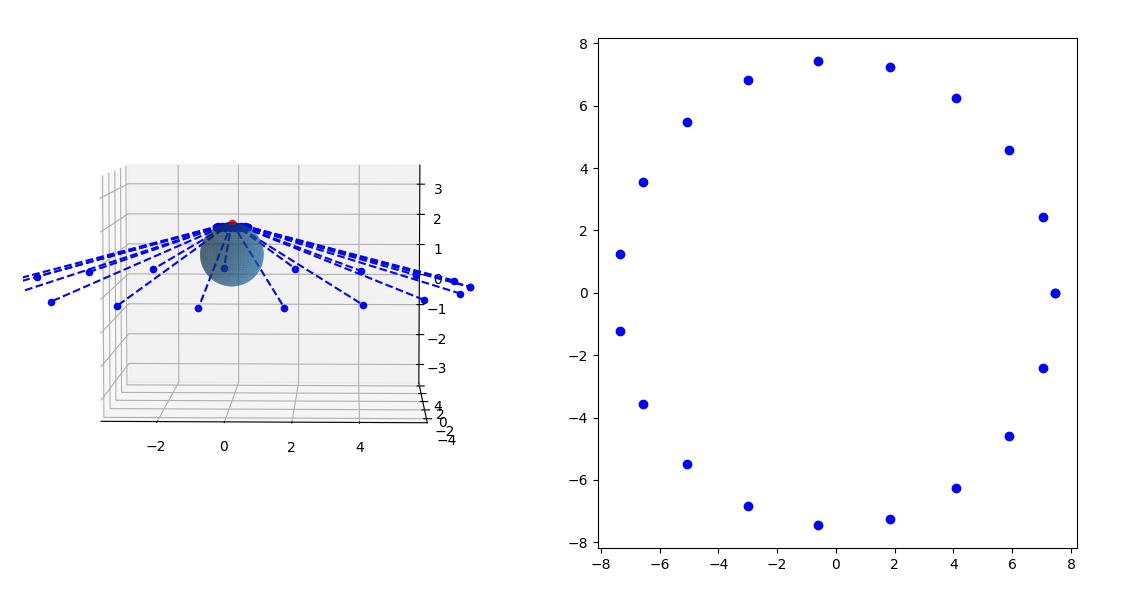
\includegraphics[width=0.8\textwidth]{Images/pi6 latitude.png}
        \end{center}

        Now the circle at $\phi = 5\pi/6$: 
        \begin{center}
        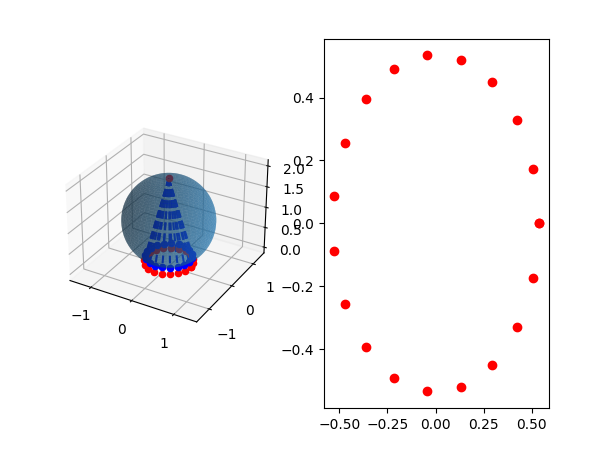
\includegraphics[width=0.8\textwidth]{Images/5pi6 latitude.png}
        \end{center}

        And finally, the circle through the North Pole ($\theta = 0$): 
        \begin{center}
        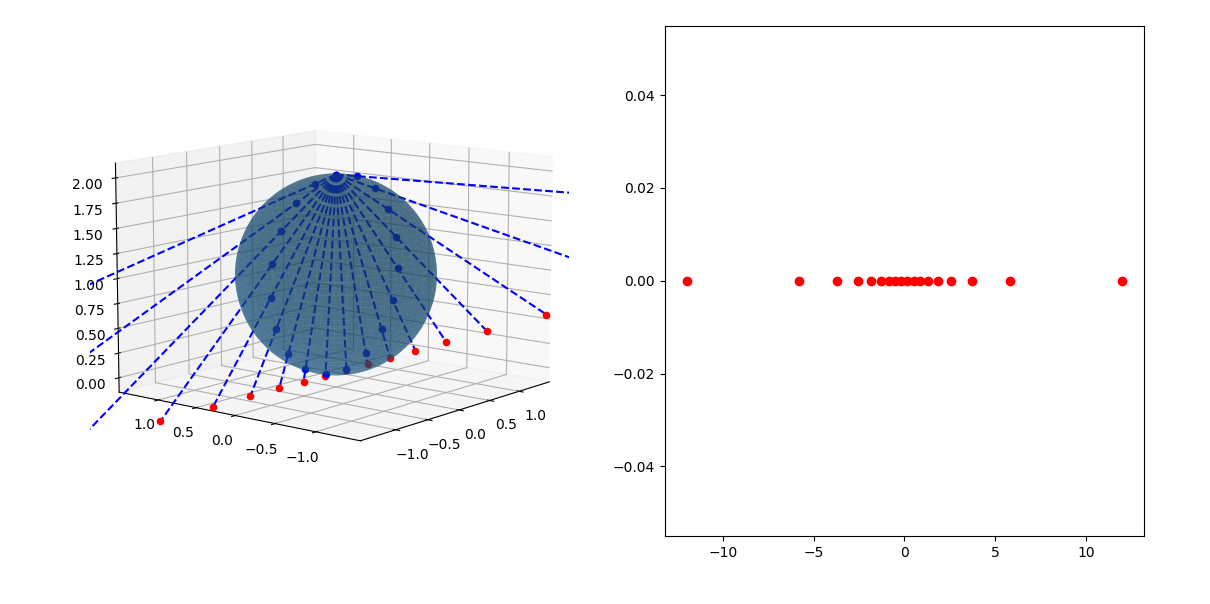
\includegraphics[width=0.8\textwidth]{Images/meridian.png}
        \end{center}
    \color{black}

\pagebreak 
5.  Given an $\alpha,\beta,\gamma \in \R$ define the function $f: \R\times \R \times \R \lra S^{2}$ via 
\[
f(\alpha,\beta,\gamma) = \left(
\begin{array}{ccc}
1 & 0 & 0 \\
0 & \cos(\alpha) &-\sin(\alpha) \\
0 & \sin(\alpha) & \cos(\alpha)
\end{array}
\right)
\left(
\begin{array}{ccc}
\cos(\beta) & 0 & -\sin(\beta) \\
0 & 1&0  \\
\sin(\beta) & 0 & \cos(\beta)
\end{array}
\right)
\left(
\begin{array}{ccc}
\cos(\gamma) & -\sin(\gamma) & 0 \\
\sin(\gamma) & \cos(\gamma) &0 \\
0 & 0 & 1
\end{array}
\right)
\left(
\begin{array}{c}
0 \\
0 \\
1
\end{array}
\right)\]
Note this function is periodic in each variable, and thus descends to a well defined function $f: S^{1}\times S^{1} \times S^{1} \lra S^{2}$ where $S^{1}$ is an angle well-defined up to an integer multiple of $2\pi$, i.e. 
$\pi/2 = \pi/2 + 2\pi k$ for each $k \in \mathbb{Z}$ inside $S^{1}$.  The angles $\alpha,\beta,\gamma$ are called $\emph{Euler angles}$ of a rotation in $\SO(3,\R)$.  Prove this map is \emph{not} a fiber bundle over $S^{2}$.  (Hint: take some derivatives)

    \color{blue}
        Suppose $f$ is a fibre bundle. Then for a small neighborhood $U \subseteq S^2$, we need $f^{-1}(U) \simeq U \times F$ for some fibre $F$.

        We can expand 
        \begin{align*}
            f(\alpha, \beta, \gamma) &= \begin{pmatrix}
                1 & 0 & 0 \\
                0 & \cos(\alpha) &-\sin(\alpha) \\
                0 & \sin(\alpha) & \cos(\alpha)
            \end{pmatrix} \begin{pmatrix} 
                \cos(\beta) & 0 & -\sin(\beta) \\
                0 & 1 & 0 \\
                \sin(\beta) & 0 & \cos(\beta)
            \end{pmatrix} \begin{pmatrix}
                0\\0\\1
            \end{pmatrix}\\
            &= \begin{pmatrix}
                1 & 0 & 0 \\
                0 & \cos(\alpha) &-\sin(\alpha) \\
                0 & \sin(\alpha) & \cos(\alpha)
            \end{pmatrix} \begin{pmatrix}
                -\sin(\beta)\\0\\ \cos(\beta)
            \end{pmatrix}\\
            &= \begin{pmatrix}
                -\sin(\beta)\\
                -\sin(\alpha) \cos(\beta)\\
                \cos(\alpha) \cos(\beta)
            \end{pmatrix}
        \end{align*}
        and take derivatives:
        \begin{align*}
            f_{\alpha}(\alpha, \beta, \gamma) &= \begin{pmatrix}
                0\\ 
                -\cos(\alpha)\cos(\beta)\\ 
                -\sin(\alpha)\cos(\beta)
            \end{pmatrix}\\ 
            f_{\beta}(\alpha, \beta, \gamma) &= \begin{pmatrix}
                -\cos(\beta)\\
                \sin(\alpha)\sin(\beta)\\
                -\cos(\alpha)\sin(\beta)
            \end{pmatrix}\\
            f_{\gamma}(\alpha, \beta, \gamma) &= \begin{pmatrix}
                0\\
                0\\
                0
            \end{pmatrix}
        \end{align*}

        But this tells us that $f$ is constant with respect to $\gamma$ so the fibre of any point in $S^2$ is a two-parameter family ($\simeq S^2$).

        Consider $N = (0, 0, 1) \in S^2$. Then $f(\alpha, \beta, \gamma) = N$ for some $\alpha, \beta, \gamma$. Indeed, we can explicitly calculate these angles: 
        \[\begin{cases}
            -\sin \beta = 0\\ 
            -\sin \alpha \cos \beta = 0\\
            \cos \alpha \cos \beta = 1
        \end{cases}\] 
        so $(\alpha, \beta, \gamma) \in \{(0, 0, \gamma), (\pi, \pi, \gamma)\}$ for any $\gamma$ which are two lines in $S^3$. 

        But, $U(N) \simeq S^1$ so as a fibre bundle, $f^{-1}(N) \simeq S^1 \times S^2$ locally. However, we have shown that the fibre is $S^2$ so this is a contradiction. 

    \color{black} 


\pagebreak 

6.  Let $\sigma: \R^{2} \lra \R^{2}$ via $\sigma(x,y) = (x+1,-y)$.  Let $\Gamma = \langle \sigma \rangle$ and consider the quotient space $Z = \R^{2}/\Gamma$.  (Recall, $Z = \R^{2}/\Gamma$ is just the space of orbits of the action of $\Gamma$ on $\R^{2}$.  Elements of $X$ may be denoted by $[(x,y)] = \{\gamma (x,y)\, | \gamma \in \Gamma \}$.  For example $\hdots [(-2,1)] = [(-1,-1)] = [(0,1)] = [(1,-1)] = [(2,1)] = \hdots$.)  

Demonstrate via picture that the map $f: Z \lra S^{1} \subset \R^{2}$ defined by
\[
f\left([(x,y)]\right) = \left( \cos(2\pi x), \sin(2\pi x) \right)
\]
is an $\R$-bundle over $S^{1}$. 

    \color{blue}
        Using Python, I generated 7 orbits starting at a random point in the range $(0, 0)$ to $(20, 20)$. The graph show the first 100 points of the orbits in $\R^2$ and their images under $f$ (shown in bright red). 

        \begin{center}
            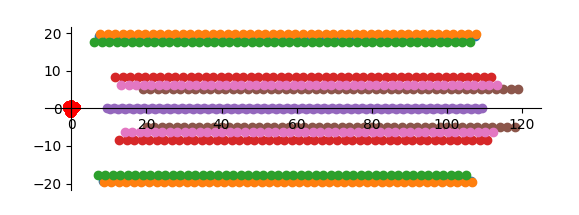
\includegraphics[width=0.8\textwidth]{Images/R bundle.png}
        \end{center}

        Clearly, for each orbit, the pre-image (fibre) is a flat line in $\R^2$ (corresponding to $\R$) and the images forms the unit circle ($S^1$). 

        Therefore, $f$ is an $\R$-bundle over $S^1$.
    \color{black}

\pagebreak 

7.  Construct the explicit fibers over the points $\hat{k}$ and $-\hat{k}$ in the Hopf-fibration as defined in class: namely the map $H : S^{3} \lra S^{2}$ defined by $H(q) = q\hat{k}q^{-1}$.  Stereographically project them into $\R^{3}$ and draw a picture of them.  Are they linked?

    \color{blue}
        We want to find $H^{-1}\{\khat\}$ and $H^{-1}\{-\khat\}$. In class we showed that for all $v \in S^2$, $H^{-1}\{v\} = qS$ where $S = \text{Stab}(\khat)$. Thus, it suffices to find a single $q \in S^3$ where $H(q) = \khat$. (or $-\khat$). 

        This amounts to finding $p \in S^3$ so that 
        \[H(p\khat) = v \implies I_p(H(\khat)) \implies I_p(\khat) = v\]
        so we can take $p\khat = q$. 

        In class we showed that for all $v \notin \{\khat, -\khat\}$, we just need to find the axis of rotation and angle $\theta$ (clockwise) from $\khat$ to $v$. 

        However, since we are now taking $v = \khat$, clearly $p = 1$. 

        And in fact this is the same as what we derived in class: Let $v = (a, b, c) = (0, 0, 1)$ then
        \[p = \frac{1}{\sqrt{2(1 + c)}}(1 + c - b\ihat + a\jhat) = \frac{1}{2}(1 + 1) = 1\]

        Therefore,
        \[\boxed{H^{-1}\{\khat\} = \text{Stab}(\khat) = \{\cos \theta + \khat \sin \theta \; | \; \theta\in [0, 2\pi]\}}\]

        However, this will not work for $-\khat$ because of division by zero. Thus, back to the rotation model: we want to find $p$ so that $I_p(\khat) = -\khat$.

        The obvious choice is any $p$ so that $p \cdot \khat = 0$. This is the $xy$-plane so we can take $p = \ihat$. Therefore, 
        \begin{align*}
            H^{-1}\{-\khat\} &= \ihat \, \text{Stab}(\khat)\\ 
                &= \ihat (\cos \theta + \khat \sin \theta)\\ 
                &= \boxed{\{\ihat \cos \theta - \jhat \sin \theta \; | \; \theta \in [0, 2\pi]\}}
        \end{align*}

        Once again using Python and the projection formula 
        \[(x, y, z) = \left(\frac{-2t}{k-2}, \frac{-2i}{k-2}, \frac{-2j}{k-2}\right)\]
        we get this image:
        \begin{center}
            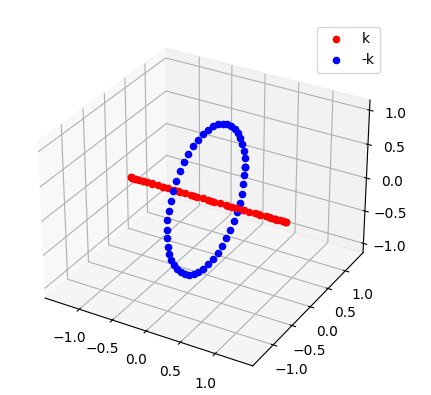
\includegraphics[width=0.8\textwidth]{Images/s3 projection.png}
        \end{center}

        So the two fibres are linked.
    \color{black}



\pagebreak 

8.  Let's say a simple closed curve is a smooth curve $\gamma: I \lra \R^{3}$ such that $\gamma$ has no self-intersections, and $\gamma(0) = \gamma(1)$.  Give two disjoint simple closed curves in $\gamma_{1}$ and $\gamma_{2}$ in $\R^{3}$, there is number one may associate called the \emph{linking number}.  If the two curves in question are unlinked, their linking number will be $0$, thus this gives us a way to distinguish certain pairs of curves as linked or unlinked.  One way to define it is via an integral.  
\[
L(\gamma_{1},\gamma_{2}) := \frac{1}{4\pi} \oint\oint_{S^{1}\times S^{1}} \frac{1}{|\gamma_{1}(s)-\gamma_{2}(t)|^{3}} \left(\frac{d\gamma_{1}}{ds}(s), \frac{d\gamma_{2}}{dt}(t), \gamma_{1}(s) - \gamma_{2}(t)\right) \, ds \, dt
\] 
where $\left( \alpha, \beta, \gamma \right)$ denotes the determinant of the vector valued curves $\alpha, \beta, \gamma$.  Calculate the linking number of the two Hopf-fibres as in Problem 7.  

    \color{blue}
        First, we need to stereographically project the fibres from Problem 7 into $\R^3$. 
       
        We have 
        \begin{align*}
            H^{-1}\{\khat\} &= \cos \theta + \khat \sin \theta \implies \gamma_1(s) = \left(\frac{\cos \theta}{1 - \sin \theta}, 0, 0\right)\\ 
            H^{-1}\{-\khat\} &= \ihat \cos \theta - \jhat \sin \theta \implies \gamma_2(t) = \left(0, \cos \theta, -\sin \theta\right)
        \end{align*}
        (since $H^{-1}\{-\khat\}$ is already in the $\ihat, \jhat$ plane).

        Because we need $\gamma(0) = \gamma(1)$, we define 
        \begin{align*}
            \gamma_1(s) &= \left(\frac{\cos(2 \pi s)}{1 - \sin(2\pi s) }, 0, 0\right)\\
            \gamma_2(t) &= \left(0, \cos (2\pi t), -\sin(2\pi t)\right)
        \end{align*}
        so 
        \[\gamma_1(0) = \gamma_1(1) = (1, 0, 0), \quad \gamma_2(0) = \gamma_2(1) = (0, 1, 0)\]
        
        Now, 
        \begin{align*}
            &L(\gamma_1, \gamma_2) = \frac{1}{4\pi} \oint \oint_{S^1 \times S^1} \frac{1}{|\gamma_1(s) - \gamma_2(t)|^3} \left(\frac{d\gamma_1}{ds}(s), \frac{d\gamma_2}{dt}(t), \gamma_1(s) - \gamma_2(t)\right)\; ds\, dt\\ 
            &= \frac{1}{4\pi} \int_{0}^{1} \int_0^1 \frac{1}{\abs{\brak{\frac{\cos(2\pi s)}{1 - \sin(2\pi s)}, -\cos(2\pi t), \sin(2\pi t)}}^3} \begin{vmatrix}
                -\frac{2\pi}{\sin(2\pi s) - 1} & 0 & \frac{\cos(2\pi s)}{1 - \sin(2\pi s)}\\ 
                0 & -2\pi\sin(2\pi t) & -\cos(2\pi t)\\
                0 & 2\pi \cos(2\pi t) & \sin(2\pi t)
            \end{vmatrix}\; ds\, dt\\ 
            &= \frac{1}{4\pi} \int_0^1 \int_0^1 \frac{1}{\abs{\brak{\frac{\cos(2\pi s)}{1 - \sin(2\pi s)}, -\cos(2\pi t), \sin(2\pi t)}}^3} \left(-\frac{2\pi}{\sin(2\pi s) - 1}\right)\left(-2\pi \sin^2(2\pi t) - 2\pi \cos^2(2\pi t)\right)\; ds\, dt\\ 
            &= \frac{1}{4\pi} \int_0^1 \int_0^1 \frac{1}{\abs{\brak{\frac{\cos(2\pi s)}{1 - \sin(2\pi s)}, -\cos(2\pi t), \sin(2\pi t)}}^3} \left(\frac{4\pi}{\sin(2\pi s) - 1}\right)\; ds\, dt\\
            &= \int_0^1 \int_0^1 \left(\frac{\cos^2(2\pi s)}{1 - 2\sin(2\pi s) + \sin^2(2\pi s)}  + \cos^2(2\pi t) + \sin^2(2\pi t)\right)^{-\frac{3}{2}} \left(\frac{1}{\sin(2\pi s) - 1}\right)\; ds\, dt\\ 
            &= \int_0^1 \int_0^1 \left(\frac{\cos^2(2\pi s)}{1 - 2\sin(2\pi s) + \sin^2(2\pi s)} + 1\right)^{-\frac{3}{2}} \left(\frac{1}{\sin(2\pi s) - 1}\right)\; ds\, dt\\ 
            &= \int_0^1 \int_0^1 \left(\frac{\cos^2(2\pi s) + 1 - 2\sin(2\pi s) + \sin^2(2\pi s)}{1 - 2\sin(2\pi s) + \sin^2 \pi s}\right)^{-\frac{3}{2}} \left(\frac{1}{\sin(2\pi s) - 1}\right)\; ds\, dt\\
            &= \int_0^1 \int_0^1 \left(\frac{2 - 2\sin(2\pi s)}{1 - 2\sin(2\pi s) + \sin^2(2\pi s)}\right)^{-\frac{3}{2}} \left(\frac{1}{\sin(2\pi s) - 1}\right)\; ds\, dt
        \end{align*} 
        \begin{align*}
            &= \int_0^1 \int_0^1 \frac{(1 - \sin(2\pi s))^3}{(2 - 2\sin(2\pi s))^{\frac{3}{2}}} \cdot \frac{1}{\sin(2\pi s) - 1}\; ds\, dt\\ 
            &= \int_0^1 \int_0^1 -\frac{\sqrt{1 - \sin(2\pi s)}}{2\sqrt 2}\; ds\, dt\\ 
            &= -\frac{1}{2\sqrt 2} \int_0^1 \int_0^1 \sqrt{1 - \sin(2\pi s)}\; ds\, dt\\
            &= -\frac{1}{2\sqrt 2} \int_0^1 \left[\frac{\sqrt{1 - \sin(2\pi s)} (\sin(\pi s) + \cos(\pi s))}{\pi(\cos(\pi s) - \sin(\pi s))}\right]_0^1\; dt\\ 
            &= -\frac{1}{2\sqrt 2}\int_0^1 \frac{2\sqrt 2}{\pi} \; dt\\ 
            &= -\frac{1}{\pi} \neq 0
        \end{align*}
        Therefore, the two fibres are linked. $\qed$ 
\color{black}


\pagebreak

\textbf{Bonus: [3 pts]}.  Let $h: S^{1}\times S^{1} \times S^{1} \lra \SO(3,\R)$ via
\[
h(\alpha,\beta,\gamma) = \left( 
\begin{array}{ccc}
1 & 0 & 0 \\
0 & \cos(\alpha) &-\sin(\alpha) \\
0 & \sin(\alpha) & \cos(\alpha)
\end{array}
\right)
\left(
\begin{array}{ccc}
\cos(\beta) & 0 & -\sin(\beta) \\
0 & 1&0  \\
\sin(\beta) & 0 & \cos(\beta)
\end{array}
\right)
\left(
\begin{array}{ccc}
\cos(\gamma) & -\sin(\gamma) & 0 \\
\sin(\gamma) & \cos(\gamma) &0 \\
0 & 0 & 1
\end{array}
\right)
\] 
Does there exist a continuous function $g: \SO(3,\R) \lra S^{1} \times S^{1} \times S^{1}$ such that $h \circ g = 1_{\SO(3,\R)}$?  \\

\textbf{Bonus: [3 pts]}.  Recall $\RP^{n}$ is defined by $S^{n}/\Z_{2}$ where $Z_{2}$ acts on $S^{2}$ via the antipodal map, $\sigma(x) = -x$.  Prove that $\RP^{3}$ is an $\RP^{1}$-bundle over $\RP^{2}$.  \\

\textbf{Bonus: [2 pts]}.  There a right $\R$-action on $\R^{2}$ via $(x,y)t:= (x,y+t)$.  Does this right $\R$-action descend to an $\R$-action on $Z = \R^{2}/\Gamma$ as in Problem 6?  Note this would imply that $Z$ is a principal $\R$-bundle over $S^{1}$.  
\end{document}